\documentclass[a4paper,12pt]{extarticle}
\usepackage[utf8x]{inputenc}
\usepackage[T1,T2A]{fontenc}
\usepackage[russian]{babel}
\usepackage{hyperref}
\usepackage{indentfirst}
\usepackage{listings}
\usepackage{color}
\usepackage{here}
\usepackage{array}
\usepackage{multirow}
\usepackage{graphicx}

\usepackage{caption}
\renewcommand{\lstlistingname}{Программа} % заголовок листингов кода

\bibliographystyle{ugost2008ls}

\usepackage{listings}
\lstset{ %
extendedchars=\true,
keepspaces=true,
language=C,						% choose the language of the code
basicstyle=\footnotesize,		% the size of the fonts that are used for the code
numbers=left,					% where to put the line-numbers
numberstyle=\footnotesize,		% the size of the fonts that are used for the line-numbers
stepnumber=1,					% the step between two line-numbers. If it is 1 each line will be numbered
numbersep=5pt,					% how far the line-numbers are from the code
backgroundcolor=\color{white},	% choose the background color. You must add \usepackage{color}
showspaces=false				% show spaces adding particular underscores
showstringspaces=false,			% underline spaces within strings
showtabs=false,					% show tabs within strings adding particular underscores
frame=single,           		% adds a frame around the code
tabsize=2,						% sets default tabsize to 2 spaces
captionpos=t,					% sets the caption-position to top
breaklines=true,				% sets automatic line breaking
breakatwhitespace=false,		% sets if automatic breaks should only happen at whitespace
escapeinside={\%*}{*)},			% if you want to add a comment within your code
postbreak=\raisebox{0ex}[0ex][0ex]{\ensuremath{\color{red}\hookrightarrow\space}},
texcl=true,
inputpath=listings,                     % директория с листингами
}

\usepackage[left=2cm,right=2cm,
top=2cm,bottom=2cm,bindingoffset=0cm]{geometry}

%% Нумерация картинок по секциям
\usepackage{chngcntr}
\counterwithin{figure}{section}
\counterwithin{table}{section}

%%Точки нумерации заголовков
\usepackage{titlesec}
\titlelabel{\thetitle.\quad}
\usepackage[dotinlabels]{titletoc}

%% Оформления подписи рисунка
\addto\captionsrussian{\renewcommand{\figurename}{Рисунок}}
\captionsetup[figure]{labelsep = period}

%% Подпись таблицы
\DeclareCaptionFormat{hfillstart}{\hfill#1#2#3\par}
\captionsetup[table]{format=hfillstart,labelsep=newline,justification=centering,skip=-10pt,textfont=bf}

%% Путь к каталогу с рисунками
\graphicspath{{fig/}}

%% Внесение titlepage в учёт счётчика страниц
\makeatletter
\renewenvironment{titlepage} {
 \thispagestyle{empty}
}
\makeatother


\begin{document}	% начало документа

% Титульная страница
\begin{titlepage}	% начало титульной страницы

	\begin{center}		% выравнивание по центру

		\large Санкт-Петербургский политехнический университет Петра Великого\\
		\large Институт компьютерных наук и технологий \\
		\large Высшая школа интеллектуальных систем и суперкомпьютерных технологий\\[6cm]
		% название института, затем отступ 6см
		
		\huge Низкоуровневое программирование\\[0.5cm] % название работы, затем отступ 0,5см
		\large Отчет по лабораторной работе №2\\[0.1cm]
		\large Программирование EDSAC\\[5cm]

	\end{center}


	\begin{flushright} % выравнивание по правому краю
		\begin{minipage}{0.25\textwidth} % врезка в половину ширины текста
			\begin{flushleft} % выровнять её содержимое по левому краю

				\large\textbf{Работу выполнил:}\\
				\large Аникин Д.А.\\
				\large {Группа:} 3530901/90004\\
				
				\large \textbf{Преподаватель:}\\
				\large Алексюк А.О.

			\end{flushleft}
		\end{minipage}
	\end{flushright}
	
	\vfill % заполнить всё доступное ниже пространство

	\begin{center}
	\large Санкт-Петербург\\
	\large \the\year % вывести дату
	\end{center} % закончить выравнивание по центру

\end{titlepage} % конец титульной страницы

\vfill % заполнить всё доступное ниже пространство


% Содержание
% Содержание
\renewcommand\contentsname{\centerline{Содержание}}
\setcounter{tocdepth}{1}
\tableofcontents
\newpage



\section{Формулировка задания}
\begin{enumerate}
\item На языке C разработать функцию, реализующую определенную вариантом задания функциональность. Поместить определение функции в отдельный исходный файл, оформить заголовочный файл. Разработать тестовую программу на языке C.
\item Собрать программу «по шагам». Проанализировать выход препроцессора и компилятора. Проанализировать состав и содержимое секций, таблицы символов, таблицы перемещений и отладочную информацию, содержащуюся в объектных файлах и исполняеммом файле.
\item Выделить разработанную функцию в статическую библиотеку. Разработать make-файлы для сборки библиотеки и использующей ее тестовой программы. Проанализировать ход сборки библиотеки и программы, созданные файлы зависимостей.
\end{enumerate}

\subsection{ Формулировка варианта задания}
Интегрирование табличной функции методом трапеций с «длинным» результатом.
\textit{Примечание: переполнение разрядной сетки предотвращается пользователем масштабированием параметра шага сетки.}

\[ \int_{a}^{b} f(x) \,dx = \sum_{i=0}^{n-1} \frac{f(x_i) + f(x_{i+1})}{2}(x_{i+1}-x_i) \]

\section{Разработка программы на языке С}
Согласно заданию, были разработаны две программы на языке С. Первая программма реализует заданную вариантом функциональность и состоит из файла с исходным кодом (libtrapz.c) и заголовочным файлом (libtrapz.h), в котором объявляется функция, являющаяся частью интерфейса вызова модуля libtrapz. Вторая программа (main.c) предназначена для тестирования работоспособности первой.
\subsection{Модуль libtrapz}
\lstinputlisting[
	label=code:hello,
	language=C,
	caption={libtrapz.c},% для печати символ '_' требует выходной символ '\'
]{libtrapz/libtrapz.c}
\parindent=1cm % командна \lstinputlisting сбивает параментры отступа

\lstinputlisting[
	label=code:bar,
	language=C,
	texcl=false,
	caption={libtrapz.h},% для печати символ '_' требует выходной символ '\'
]{../include/libtrapz/libtrapz.h}
\parindent=1cm % командна \lstinputlisting сбивает параментры отступа

\subsection{Модуль app}
\lstinputlisting[
	label=code:hello,
	language=C,
	caption={main.c},% для печати символ '_' требует выходной символ '\'
]{app/main.c}
\parindent=1cm % командна \lstinputlisting сбивает параментры отступа

\section{Сборка программы ''по шагам''}
\subsection{Препроцессирование}
Первым шагом является препроцессирование файла исходного текста. На данной стадии происходит происходит работа с препроцессорными директивами. Например, препроцессор добавляет хэдеры в код (\textbf{\#include}), убирает комментирования, заменяет макросы (\textbf{\#define}) их значениями, выбирает нужные куски кода в соответствии с условиями \textbf{\#if}, \textbf{\#ifdef} и \textbf{\#ifndef}. 

\makeatletter
\def\lst@PlaceNumber{\llap{\normalfont
                \lst@numberstyle{\the\lst@lineno}\kern\lst@numbersep}}
\makeatother

\lstinputlisting[
	label=code:hello_mod,
	linerange={1-6, 23-33},
	texcl=false,
	basicstyle=\tiny,
	caption={Фрагмент libtrapz.i},
]{../doc/listings/libtrapz.i}
\parindent=1cm

\lstinputlisting[
	label=code:ww,
	linerange={1-6, 1282-1296},
	texcl=false,
	basicstyle=\tiny,
	caption={Фрагмент main.i},
]{../doc/listings/main.i}
\parindent=1cm

В новых сгенерированных файлах можно увидеть огромное количество новых строк, в основном ''хедеры'' \textbf{<stddef.h>} и \textbf{<stdio.h>}. Появившиеся нестандартные директивы, начинающиеся с символа ''\#'', используются для передачи информации об исходном тексте из препроцессора в компилятор.

\subsection{Компиляция}
На данном шаге компилятор выполняет свою главную задачу — компилирует, то есть преобразует полученный на прошлом шаге код без директив в ассемблерный код. Рассмотрим полученные файлы libtrapz.s и main.s

\lstinputlisting[
	label=code:wwe,
	texcl=false,
	caption={libtrapz.s},
]{../doc/listings/libtrapz.s}
\parindent=1cm

Особый интерес представляет форма хранения чисел с плавающей запятой двойной точности: целая и дробная часть числа хранятся раздельно в формате word. Для взаимодействия с ними используются внутренние специальные функции, такие как \textit{\_\_adddf3}. В метке .L3 хранится код для вычисления по формуле. Метка .L1 отвечает за возвращение результата выполнения и выход из программы. 
\newline
\newline

\lstinputlisting[
	label=code:wwe,
	texcl=false,
	caption={main.s},
]{../doc/listings/main.s}
\parindent=1cm

Видно, что тестовая программа вызывает функцию trapz, аргументы передаются через регистры a0, a1, a2. В метке .LC1 хранится массив Y, а в .LC0 - массив X.

\subsection{Ассемблирование}
Ассемблер преобразовывает ассемблерный код в машинный код, сохраняя его в объектном файле. Сформированный ассемблером объектный файл должен содержать коды инструкций, таблицу символов и таблицу перемещений. В отличие от ранее рассмотренных файлов, объектный файл не является текстовым, для изучения его содержимого используется утилиту objdump, отображающая содержимое бинарных файлов в текстовом виде.

Изучим содержимое таблиц символов объектных файлов.
\lstinputlisting[
	label=code:wwe,
	texcl=false,
	caption={Таблица символов libtrapz.o},
]{../doc/listings/libtrapz_symdump.txt}
\parindent=1cm

\lstinputlisting[
	label=code:wwe,
	texcl=false,
	caption={Таблица символов main.o},
]{../doc/listings/main_symdump.txt}
\parindent=1cm

В таблице символов  имеется интересные записи: симвоы типа “*UND*” (undefined – не определен).
Эти записи означают, что символ использовался в ассемблерном коде, из которого был
получен данный объектный файл, но не был определен; ассемблер сделал вывод о том, что
символ должен быть определен где-то еще, и отразил это в таблице символов.

Изучим содержимое секции “.text” объектных файлов.

\lstinputlisting[
	label=code:wwe,
	texcl=false,
	caption={Инстркци программы},
]{../doc/listings/objdump.txt}
\parindent=1cm

Интерес представляет трансформация псевдоинструкции call, а именно странные переходы на предыдущую инструкцию. Поведение ассемблера объясняется очень просто: ассемблер не имел возможности определить целевой адрес перехода, поэтому не мог сформировать корректную инструкцию передачи управления. В
результате была сформирована пара инструкций с некорректными  значениями епосредственных операндов. Для получения исполняемого кода эта пара инструкций должна быть исправлена компоновщиком.

Информация обо всех «неоконченных» инструкциях передается ассемблером компоновщику
посредством таблицы перемещений.

Для того чтобы внести необходимые исправления, требуется знать, что исправить, как исправить и
какой символ следует использовать, именно эта информация и содержится в записях о
перемещениях.

\lstinputlisting[
	label=code:wwe,
	texcl=false,
	caption={Таблица перемещений},
]{../doc/listings/rdump.txt}
\parindent=1cm

Так, например, указано, что по адресу 68 следует
исправить пару инструкций (тип перемещения ''R\_RISCV\_CALL'') так, чтобы результат
соответствовал вызову подпрограммы \_\_adddf3.

\subsection{Компоновка}
Компоновщик связывает все объектные файлы и статические библиотеки в единый исполняемый файл, который мы и сможем запустить в дальнейшем. Изучим содержимое секции “.text” полученного в результате компоновки программы
исполняемого файла. 

Выходной файл содержит значительно больше строк, чем было до этого (20000!). Это связано с включением стандартной библиотеки при компоновке. Нас интересует лишь небольшой отрывок.

\lstinputlisting[
	label=code:wew,
	linerange={152-159, 196-197},
	texcl=false,
	caption={Фрагмент дизасемблированного файла},
]{../doc/listings/linkeddump.txt}
\parindent=1cm

Как видно, адресса были скорректированы компоеновщиком, при этом адрессация изменилась на абсолютную. 

\section{Создание статической библиотеки}
Статическая библиотека является, по сути, архивом объектных файлов, среди которых компоновщик выбирает «полезные» для данной программы:объектный файл считается «полезным», если в нем определяется еще не разрешенный компоновщиком символ.

Рассмотрим список сиволов библиотеки ''libtrapz.a''

\lstinputlisting[
	texcl=false,
	caption={Список символов библиотеки},
]{../doc/listings/nmdump.txt}
\parindent=1cm

Несложно догадаться, что в выводе утилиты “nm” кодом “T” обозначаются символы,
определенные в соответствующем объектном файле, кодом “U” - внешние символы.

Используем статическую библиотеку для сборки программы и изучим таблицу символов исполняемого файла.

\lstinputlisting[
	label=code:ww,
	linerange={115-127},
	texcl=false,
	caption={Фрагмент дизасемблированного файла},
]{../doc/listings/dumplib.txt}
\parindent=1cm

Убеждаемся, что там находится наша функция.

\section{Автоматизация процесса сборки}
Для автоматизации сборки библиотеки и тестируемой программы был написан Makefile.

\lstinputlisting[
	label=code:ww,
	texcl=false,
	caption={../Makefile}
]{../Makefile}
\parindent=1cm

В результате сборки была собрана статическая библиотека libtrapz.a и исполняемый файл тестируемой программы ''trapz''. Объектные файлы хранятся в дирректории build (Рисунок 5.1 ).

\begin{figure}[H]
	\begin{center}
		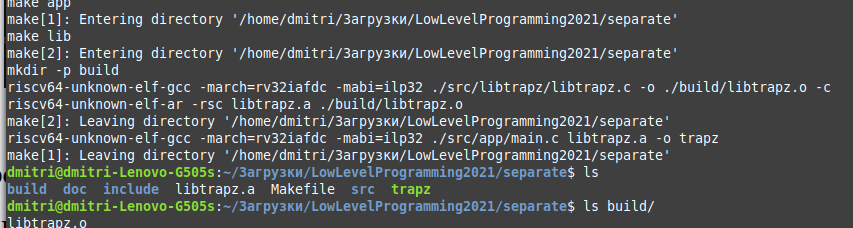
\includegraphics[scale=0.5]{1}
		\caption{Результат сборки программы} 
		\label{pic:pic_name} % название для ссылок внутри кода
	\end{center}
\end{figure}

\section{Проверка работоспособности}
Для проверки работоспособности программ, они были собраны тулчейном x86\_64. Результат выполнения приведен на рис. 6.1

Тестирующая программа находит значение определенного интергала для заданной табличной функции:
\begin{table}[H]
	\caption{Заданная табличная функция}
	\begin{center}
		\begin{tabular}{|l|l|l|l|l|l|}
			\hline
			X  & 1.1 & 2.28 & 4.6 & 5    & 10.001\\ \hline
			Y  & 0.8 & 0.16 & 0.8 & 0.16 & 0.8\\ \hline
		\end{tabular}
		\label{tabular:tab_examp}
	\end{center}
\end{table}

\begin{figure}[H]
	\begin{center}
		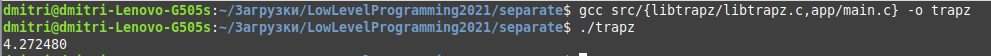
\includegraphics[scale=0.5]{2}
		\caption{Результат выполнения программы} 
		\label{pic:pic_name} % название для ссылок внутри кода
	\end{center}
\end{figure}

Проверим верность результата, вызвал аналогичную функцию в среде Matlab

\begin{figure}[H]
	\begin{center}
		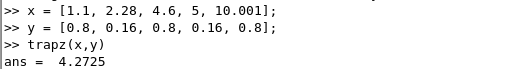
\includegraphics[scale=0.5]{3}
		\caption{Результат функции в среде Matlab} 
		\label{pic:pic_name} % название для ссылок внутри кода
	\end{center}
\end{figure}

\section{Выводы}
В ходе выполнения лабораторной работы была разработана программа на языке C, реализующая заданную функциональность. Была осуществлена сборка программы по шагам для ISA RV32I, проанализированы выводы препроцессора, компилятора, компоновщика. 
Создана статическая библиотека libtrapz.a, на основе которой собрана тестирующая программа. Для автоматизации сборки был разработан Makefile с павилами сборки.
\end{document}
